%# -*- coding: utf-8-unix -*-
%%==================================================
%% chapter01.tex for SJTU Master Thesis
%%==================================================

\chapter{绪论}
\label{chap:intro}

本章首先介绍模拟集成电路设计的概况,指出其设计过程中由于计算机辅助设计的缺失带来的设计效率低下的问题。
进而回顾符号化分析方法在这一问题上所作出的诸多努力,并简要介绍并比较相应成果。
最后介绍本文的主要内容,并给出文章组织安排。

\section{模拟集成电路设计方法概述}
\label{sec:intro:analog}
随着半导体产业的不断发展与电子设备的不断的推陈出新,对集成电路设计的时效性及高效性提出了更高的要求。
同时,越来越多的功能被集成在同一块芯片内部,从而推动了SoC(System-on-Chip)概念的形成,对电路设计带来更多困难与挑战\parencite{Saleh-SoC-2006}。
作为集成电路设计的两大重要分支,数字集成电路设计和模拟集成电路设计的设计方法决定了SoC设计效率,同时保证了电路性能与可靠性。
其中,由于电子设计自动化(Electronic Design Automation, EDA)工具的成熟,数字集成电路设计的效率已远远超过模拟电路设计\parencite{Ghasi-VLSID-2009}。
数字电路在整个设计流程,如电路综合、验证、自动布局布线等,均有对应的EDA工具做相应的支持。
除此之外,数字集成电路中由于有IP(Intellectual Property)核的支持,可以轻松地对功能模块进行重用,大大方便了数字电路工程师进行电路设计。
然而相对应的,模拟电路由于其电路性能特征描述的困难以及针对不同应用设计变化复杂等原因一直导致其IP化进程并不十分顺利\parencite{Zheying-ICASIC-2003, Saleh-SoC-2006}。

\begin{figure}[!htp]
	\centering
	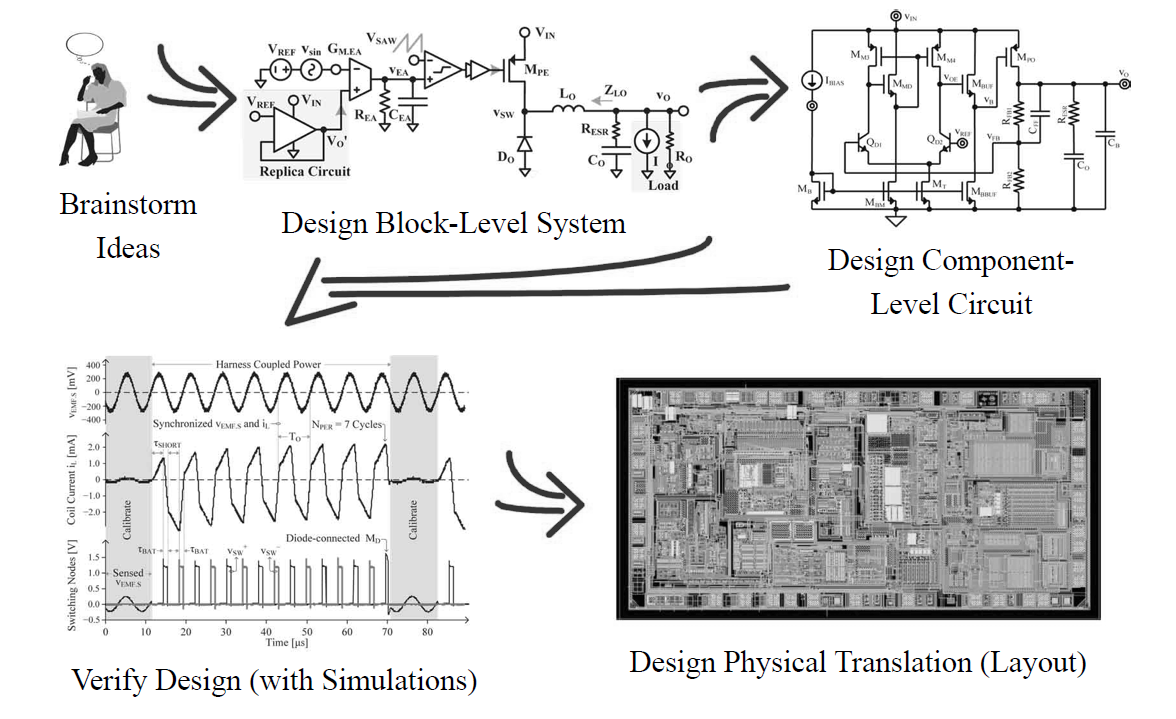
\includegraphics[width=0.9\textwidth]{chap1/AICWhy.png}
	\bicaption[fig:AICWhy]{基本模拟集成电路设计流程}{基本模拟集成电路设计流程\parencite{Gabriel-AICWhy}}{Fig}{Basic analog integrated circuits design procedure \parencite{Gabriel-AICWhy}}
\end{figure}

模拟集成电路在现代SoC设计中基本只占这个芯片面积的10\%-50\%,然而这个设计流程中有近50\%-90\%的时间用于模拟部分的设计与测试\parencite{Gabriel-AICWhy}。
而且往往由于模拟电路的设计错误,可能导致多次流片验证,增加了设计成本。
模拟集成电路自与1964年诞生以来\parencite{Thomas-AICHistory-2007},基本一直遵循图\ref{fig:AICWhy}中的设计流程。
电路设计往往从整体系统建模开始,然后根据系统的整体性能指标,给出更具体的电路功能模块的性能指标。
然后,参照模块性能,选择合适的电路结构,并结合电路仿真结果,确定元件参数。
综合所有功能模块,在完成系统层面仿真。
最后,手工绘制版图后,并检查无误后,送至工艺厂进行生产。
由于上述设计流程限制,模拟电路设计往往受到以下条件制约:

\begin{enumerate}[label=\emph{\alph*})]
	\item 上述大部分流程均为人工计算设计得到,缺乏计算机辅助设计流程,大部分情况下需要工程师的个人经验作为设计依据。
	\item 上述流程往往需要多次反复,根据仿真结果一再调整结果,带来设计效率的低下。
	\item 模拟电路仿真往往花费大量时间,特别是在系统级的仿真中,任何参数的调整带来巨大的时间损耗,拉长了整个设计周期。
\end{enumerate}

可以看到,上述原因主要是由于模拟电路设计缺乏计算机辅助设计工具,导致设计方法因人而异,没有形成系统化的设计体系所造成的。
其中,模拟电路的建模是关键的一环。
如果存在系统化自动化的模拟电路建模方法,那么首先由于模型的建立方式的统一,会带来设计人员学习理解的方便。
同时,由于所建立的电路模型中可以带有电路元件参数,直接将电路性能与电路元件取值联系在一起,方便了电路设计的优化流程。
另外,自动化建模可以在系统仿真层面大大加快设计效率,提升仿真速度。
故可以看到提出行之有效的系统化自动化模拟电路建模方案将在一定程度上有效地解决上述三个制约条件,对加快电路设计效率有着至关重要的作用。

\section{符号化分析方法}
\label{sec:intro:symbolic}

目前,模拟电路仿真主要采用以SPICE为基础的数值化仿真工具\parencite{Nagel-SPICE-1973},如Cadence公司的Spectre以及Synopsys的HSPICE仿真器等。
数值仿真器以其稳定高效的数值求解结果成为业界的常用仿真工具。
然而数值仿真方法最大的问题在于其仿真结果与电路元件参数的取值脱节,很难从电路的仿真结果对电路元件的取值反推相应的结果。
这导致电路工程师,特别是经验不丰富的工程师,在不确定电路元件与性能关系的情况下,只能对电路元件取值进行盲目的调整,以期达到所要求的性能指标。
为了克服这一困难,本文采用符号化仿真方法对电路进行分析。

\subsection{符号化分析方法回顾}
\label{subsec:intro:symbolic:review}

上世纪90年代,另一种电路仿真方法符号化仿真方法得到了许多关注\parencite{Lin-Symb}。
与数值化仿真不同,符号化仿真方法会直接建立小信号电路传输函数与电路元件之间的表达式,然后通过所求的电路传输函数表达式进行求解,如图\ref{fig:symbolic}所示的流程。

\begin{figure}[!htp]
	\centering
	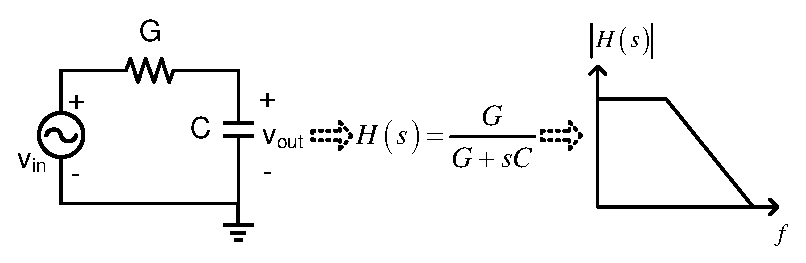
\includegraphics[width=0.7\textwidth]{chap1/symbolic.eps}
	\bicaption[fig:symbolic]{符号化分析流程}{符号化分析流程}{Fig}{General symbolic analysis procedure}
\end{figure}

这种电路分析方式带来诸多数值化仿真不能得到的好处,主要可以归纳为以下几点:

\begin{enumerate}[label=\emph{\alph*})]
	\item 可以直观地通过符号化公式告知电路设计者所有电路元件参数对电路的作用,有助于工程师进行优化调整及相应的分析。
	\item 在构造解析表达式后,在电路元件重新调整后,可以直接通过得到的公式进行仿真求解,避免费时的数值矩阵迭代过程。
	\item 可以通过求解得到的公式对电路进行表征,构建相应的电路模型,用于将来的模拟电路功能模块综合、验证等功能的实现。
\end{enumerate}

构建符号化表达式十分多样,过去开发了多种不同的符号化求解方式,如矩阵行列式展开求解\parencite{Gielen-ISAAC-1989}、利用Mason规则求解信号流图\parencite{Nebel-SFG-1995,Fino-SFG-1998}、双图枚举\parencite{Shieu-TG-1974}等。
这些算法都可以求解一个线性电路的传输函数;针对如含有MOSFET的非线性电路,求解器则会通过静态工作点仿真得到非线性元件的小信号模型,并带入计算。

然而,由于符号化分析方法本身性质决定,随着电路规模的增长,符号化分析中符号化项的规模也呈指数级增长,\parencite{Gielen-SymbSurvey-1998}对各种不同的符号化方法中的规模增长进行了验证与比较。
这在很大程度上限制了符号化方法在大规模电路中的应用,甚至当时提出的多数算法难以对一个完整的运放电路进行符号化分析。
其次多数符号化方法,与节点分析法、回路分析法等传统电路分析方法差异比较大,很多算法都存在规则繁琐,不利于手工计算的问题,所以相对其推广也更加不如数值化分析方法。

\subsection{双图决策树(GPDD)符号化分析方法}
\label{subsec:intro:symbolic:gpdd}

为解决符号化表达式增长过快的问题,Sheldon X.-D. Tan于2000年附近提出了DDD(Determinant Decision Diagram)符号化方法。
他们使用Cramer法则计算电路传输函数,并利用二分决策图(Binary Decision Diagram, BDD)结构\parencite{Bryant-BDD-1986}来存储计算过程中得到的符号化表达式\parencite{Sheldon-DDD-2000}。
这种方法有效地缓解了符号化公式占用大量存储空间的问题,但是其所保存的符号化公式存在非常多的对消项。(对消项会在第\ref{chap:simp}章有更详细的描述。)
这造成了计算机计算过程中的数值误差的累积,其求解结果有一定误差。

2006年附近,G. Shi等人提出了双图决策树(Graph-Pair Decision Diagram, GPDD)方法\parencite{ChenWeiWei-Thesis,GShi-GPDD-2013,GShi-GPDD,GShi-GPDDSurvey-2013}。
此方法也利用了BDD结构,对符号化项进行隐式枚举,从而保证了与DDD相当的高效的空间利用率。
虽然,这种方法的符号化结果规模仍然随着电路规模呈指数级增长,但是由于相较早期的符号化方法,其增长速度较慢,以足以分析一个运放这样规模的电路。
同时,该方法从理论保证了对消项不会在最终得到的符号化表达式中出现,从而可以得到非常精确的计算结果。

近几年来,GPDD方法从软件实现仿真到电路建模优化等多方面得到了许多发展。
\parencite{XuHui-Hier-2011, LiXiaopeng-Hier-2011, SongYang-Hier-2012}中使用了层次化的方法,从而实现了对较大规模模拟集成电路的分析;
\parencite{MengXiaoxuan-Sens-2009,WengBinbin-Sens-2011,ChenJiajun-Sens-2012}中利用符号化敏感度分析方法,对电路元件敏感性进行了探索,并开发了自动调整运放尺寸的算法;
\parencite{ZhangHe-Slew-2011,ZhangAilin-Slew-2015}通过Moment Matching的方法对电路零极点进行建模,从而得到运放时域电路模型;
\parencite{ChengJiandong-SC-2013}实现了对开关电容电路的仿真,从而得到了z域的GPDD仿真方法;
\parencite{ChengJiandong-SDM-ASPDAC-2013, ChengJiandong-SDM-TENCON-2013}进一步将其应用到Sigma-Delta调制器中。

下面通过一例子对这种方法进行详细介绍。

\begin{exmp}
RC电路的GPDD构造示例
	
考虑如图\ref{fig:RC_cir}所示的RC低通滤波器电路,这里希望求取电路的从输入电压至电容两端输出电压的传输函数。
根据电路结构,构造如图中右侧所示的图,将电路元件抽象为图中的边,用电路元件的导纳值作为元件的符号。
其中电路的输入输出关系,我们用从输出控制输入的受控源$X$来进行标识,并作为GPDD结构的根节点。
这里由于是输出电压控制输入电压,故为电压控制电压源(VCVS),在图中即为对应的紫色VC和VS边。
	
\begin{figure}[!htp]
	\centering
	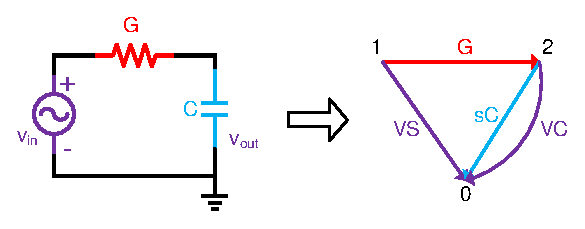
\includegraphics[width=0.6\textwidth]{chap1/RC_cir.eps}
	\bicaption[fig:RC_cir]{RC低通滤波电路及对应原始图}{RC低通滤波电路及对应原始图}{Fig}{RC low-pass filter \& its corresponding graph}
\end{figure}

根据双图电路分析理论\parencite{Lin-Symb},可以知道在上述电路中可被接受的生成树对仅有图\ref{fig:RC_tree}中所示的三对,同时每一个生成树对构成了一个符号化的项。
如将这些项相加,并使它等于0,则可求得电路的传输函数:

\begin{equation}
\label{eq:RC}
- XG + G + sC = 0 \Rightarrow H\left( s \right) = \frac{1}{X} = \frac{G}{G + sC}
\end{equation}

\begin{figure}[!btp]
	\centering
	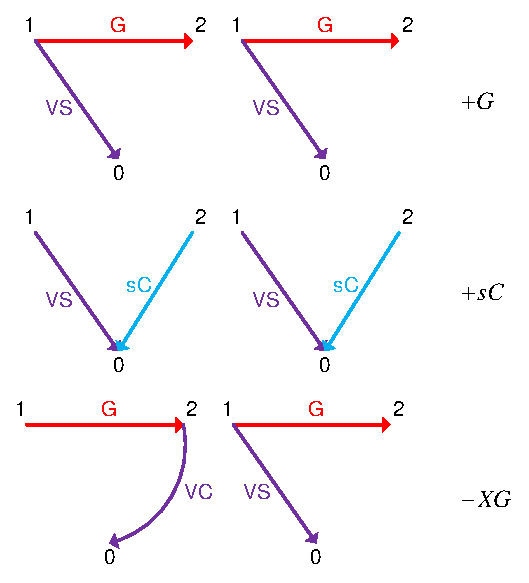
\includegraphics[width=0.55\textwidth]{chap1/RC_tree.eps}
	\bicaption[fig:RC_tree]{RC低通滤波电路生成树对}{RC低通滤波电路生成树对}{Fig}{Spanning tree pairs in RC low-pass filter}
\end{figure}

为了能够快速枚举原始图中所有的符合条件的生成树对,GPDD算法是用了类似图\ref{fig:RC_GPDD}所示的BDD结构来保存枚举结构\parencite{GShi-GPDD-2013}。
GPDD结构每一层有且仅有一个元件符号,每个GPDD节点有两个2儿子,左儿子用实线与下面的节点连接,右儿子用虚线与下面的节点连接。
不同节点可以共享同一个儿子,这也是GPDD之所以可以用较少空间存储大量符号化项的原因,类似于多项式的公因式提取。
所有的节点必然终结于$1$结点或$0$结点。
可以看到这个GPDD结构中共有3条从根节点通往$1$结点的路径,如路径经过了实线,那么实线出发点的符号会出现在该符号项中;如是虚线,则不出现。
经验证,可知道这3条路径正是指代前面的3个生成树对,从而可以保存了电路的传输函数的符号化表达。

\begin{figure}[!htp]
	\centering
	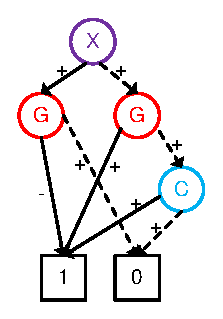
\includegraphics[width=0.2\textwidth]{chap1/RC_GPDD.eps}
	\bicaption[fig:RC_GPDD]{RC电路的GPDD结构示例}{RC电路的GPDD结构示例}{Fig}{GPDD structure of RC circuit}
\end{figure}

\begin{figure}[!htp]
	\centering
	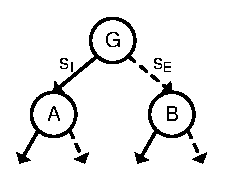
\includegraphics[width=0.25\textwidth]{chap1/evalGPDD.eps}
	\bicaption[fig:evalGPDD]{GPDD求值规则}{GPDD求值规则}{Fig}{The evaluation rule for GPDD}
\end{figure}

这里简要介绍GPDD结构的计算方法。如图\ref{fig:evalGPDD}所示,对于GPDD结构中某个节点$G$的求值,用$f_{G} \left( G \right)$来标示。
在递归得求得其左右子GPDD结构的值后,用其符号本身$G$乘以以实现相连的$A$节点的值$f_{A} \left( A \right)$,并加上虚线相连的$B$节点的值$f_{B} \left( B \right)$。
注意这里,需记得考虑实线及虚线上所标识的符号$s_I$和$s_E$,$s_I$和$s_E$仅为正负关系。总结可如下式所示:

\begin{equation}
\label{eq:evalGPDD}
f_{G} \left( G \right) = s_I G f_{A} \left( A \right) + s_E f_{B} \left( B \right)
\end{equation}

如使用式\ref{eq:evalGPDD}可以验证得到式\ref{eq:RC}的结果。
根据该计算规则,可以通过自底向上遍历整个GPDD结构,求得电路传输函数。
在根节点处,无需显式求解令方程等于0的传输函数值。
假设根节点$X$左儿子为$N$,符号为$s_N$;右儿子为$D$,符号为$s_D$。那么电路传输函数即为:

\begin{equation}
\label{eq:evalGPDDRoot}
s_N  X f_N\left(N\right) + s_D f_D\left(D\right) = 0 \Rightarrow H \left( s \right) = \frac{1}{X}= - s_N s_D \frac{f_N\left(N\right)}{f_D\left(D\right)}
\end{equation}

\end{exmp}

\section{电路模型符号化简化方法简介}
\label{sec:intro:simp}

另一方面由于符号化的

\subsection{构建前简化方法}
\label{subsec:intro:simp:SBG}
\parencite{Hsu-SBG-1994}
\subsection{构建中简化方法}
\label{subsec:intro:simp:SDG}
\parencite{Fern-SDG-1994}
\subsection{构建后简化方法}
\label{subsec:intro:simp:SAG}
\parencite{Zivkovic-TopoSimp-1995,Sheldon-DDDSimp-1999}

\subsection{符号化模型降阶}
\label{subsec:intro:symbolic:smor}
\parencite{GShi-SMOR-2006}

\section{主要贡献与章节安排}

\label{sec:intro:org}